% \begin{abstract}

% Tensor kernels in machine learning (ML)
%   often correspond to pure mathematical expressions,
%   making term rewriting an attractive strategy
%   for optimization and mapping to specialized hardware accelerators.
% %   ---%
% %   especially given recent progress in equality saturation.
% However,
%   existing ML intermediate representations (IRs)
%   tend to either be \textit{pure but high-level},
%   making low-level rewrites
%   to hardware targets inexpressible,
%   or \textit{low-level but impure},
%   hampering the use of term rewriting altogether.
% %   leaving no suitable IR
% %   for term rewriting
% %   over low-level tensor kernels.

% This paper introduces \g,
%   a pure IR whose core abstraction---%
%   the \textit{access pattern}---%
%   enables
%   low-level,
%   layout-aware,
%   hardware-centric
%   program rewrites.
% We demonstrate how term rewriting
%   in \g
%   can be used to 
%   map program fragments
%   to hardware accelerator invocations
%   and
%   automatically discover
%   classic data layout transformations
%   like \tcd{im2col}.
% % Hm... not capturing this idea at the moment:
% %  that facilitate hardware--software mapping
% %  but previously required explicit manual implementation.
% \g establishes a new foundation for
%   exploring further term rewriting techniques
%   in optimizing low-level tensor programs.
% %  \hl{todo we don't ever explain hardware--software programs}



% \end{abstract}

\chapter{Glenside}
\label{sec:part1-glenside}

\textit{This is derived from the work done in \ref{glenside}.}

\section{New Introduction}

In the previous chapter,
  we laid out our need
  for a system
  which can allow us
  to reason about tensor programs efficiently.

Equality saturation is this thing
  that has these benefits.

However, equality saturation requires
  a pure representation.
Also it doesn't like binding.

Hence we introduce \g.


\section{Introduction}

\hl{should this stuff be moved up to 3LA?}

Machine learning (ML) and other
  high-performance computing (HPC)
  applications increasingly rely on
  specialized hardware accelerators to
  provide speed and energy efficiency~\cite{jouppi2017tpu, krizhevsky2012conv, reuther2019survey}.
This trend has highlighted the need
  for flexible accelerator support
  in domain-specific compilers like
  Halide~\cite{halide},
  TVM~\cite{chen2018tvm},
  TensorFlow/MLIR~\cite{tensorflow, mlir}, and
  PyTorch~\cite{pytorch}.

Adding accelerator support to
  an existing compiler typically
  uses custom pattern matching to
  map expensive tensor operations
  from applications down to
  accelerator invocations~\cite{
    yang2020interstellar, byoc}.
Pattern matching often additionally relies on
  various other transformations
  to canonicalize intermediate representations (IRs)
  %~\cite{??}
  and massage data layouts into
  formats matching accelerator requirements~\cite{nvidia2020nhwc}.
Even with these changes,
  users may need to manually modify their application to
  help the compiler discover opportunities
  for dispatching operations to accelerators, 
  such as by changing data types or unrolling loops.
    
In principle, term rewriting techniques~\cite{baader1998term}
  should be able to facilitate many of
  these transformation and mapping tasks
  within a compiler.
Halide and TVM already rely
  on extensive rewrite systems for
  optimizing scalar computations and
  simplifying loop bounds in order to
  support further downstream optimizations~\cite{newcomb2020halide-rewrite,
  hagedorn2020func-high-perf}.

Unfortunately, existing IRs in compilers for
  array/tensor programming DSLs tend to
  present abstraction and granularity mismatches
  that hamper term rewriting approaches.
Term rewriting is most easily applied in
  \textit{pure} (side effect--free) IRs
  that support equational reasoning.
At the same time,
  mapping to accelerators requires considering
  low-level hardware details like data layout.
Existing pure IRs for ML frameworks are used
  primarily for high-level transformations
  (e.g., type elaboration and inlining)
  and do not expose low-level data layout details~\cite{relay}.
On the other hand,
  IRs used for crucial lower-level optimizations like
  operator fusion must support
  precise reasoning about memory use,
  and therefore are typically impure,
  hampering term rewriting.% approaches.

To help mitigate such impedance mismatches,
  we present \textit{\g},\footnote{Publicly available at \url{https://github.com/gussmith23/glenside}.}
  a pure tensor program IR
  that enables hardware-level term rewriting.
\g is based on a simple
  \textit{access pattern} abstraction that
  supports expressing and reasoning about
  data layout transformations via
  syntactic rewrite rules.
% We moved this figure elsewhere in the thesis
%   \begin{wrapfigure}{r}{.5\textwidth}
%     \centering
%     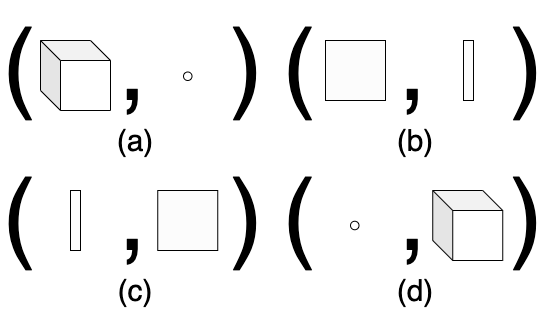
\includegraphics[width=.9\linewidth]{glenside/access-pattern-examples-2x2.png}
%     \caption{
%       Four access patterns,
%         representing different ways
%         a
%         tensor program
%         (or \textit{kernel})
%         might access
%         the same 3D tensor. 
%       For example, (c) represents
%         accessing a 3D tensor as
%         a vector of 2D matrices.}
%     \label{fig:access-pattern-examples}
%     \vspace{-1em}
% \end{wrapfigure}
When combined with standard arithmetic rewrites
  for per-tensor-element computations,
  access patterns enable implementing complex
  transformations for accelerator support as
  compositions of simple rewrites.

Tensors are traditionally characterized
  by their \textit{shape},
  an $n$-tuple 
  %in $\mathbb{N}^n$
  of positive integers
  indicating the size of each
  of a tensor's dimensions.
  % , e.g., $(x, y, z)$ for a 3D tensor.
Access patterns instead characterize
  each tensor with two shapes, e.g.,
  \accesspatternshape{x}{y, z}, separating
  the dimensions which are \textit{iterated over} from
  the dimensions which are \textit{computed on.}
Figure~\ref{fig:access-pattern-examples}(c)
  depicts an example where a 3D tensor's
  first dimension is iterated over and
  some computation applied to each
  corresponding 2D matrix.

We demonstrate how \g
  enables implementing representative
  hardware-level transformation via term rewriting,
  including mapping computations
  to systolic arrays~\cite{jouppi2017tpu}
  (a common hardware module in ML accelerators)
  and automatically discovering the
  \tcd{im2col} data layout transformation~\cite{im2col},
  which enables mapping 2D convolutions
  to matrix multiplication hardware.
In particular,
  by employing \textit{equality saturation}~\cite{willsey2021egg},
  these transformations ``fall out for free''
  (i.e., without any carefully crafted
  rewrite orderings~\cite{phase-ordering}),
  from a handful of general rewrites concerning tensor
  transposition, Cartesian product, dot product, etc.,
  expressed in terms of access patterns.

To summarize, the contributions of this chapter include:
\begin{itemize}
\item \textit{Access patterns},
  a tensor representation that employs a
  simple, extended tensor shape type to
  distinguish iteration and computation dimensions

\item The \g IR,
  a pure compiler IR that facilitates 
  term rewriting to enable support for
  specialized accelerators
  
\item A library of generic rewrites over \g programs
  
% \item Case studies demonstrating how
%   \g enables automatically discovering
%   key transformations for mapping
%   applications to custom accelerators
%   via equality saturation with the
%   \tcd{egg}~\cite{willsey2021egg} library.
\end{itemize}

\hl{i moved related work, so probably need to rework this}
The rest of this chapter is organized as follows:
Section~\hl{todo} provides background
  and briefly surveys closely related work.
Section~\hl{todo} motivates
  \g via a running example exploring
  pure matrix multiplication.
Section~\hl{todo} details the
  design and implementation of \g.


\section{From Pure \texttt{matMul} to IR Design Goals}
\label{sec:matmul}

% Many ML and HPC workloads are dominated by
%   evaluating compositions of tensor algebra operators
%   which, at a high level, correspond to
%   pure mathematical expressions.
% This make functional programming techniques attractive,
%   but requires careful design to ensure that
%   nested operators remain compositional with
%   respect to their output shapes.
% To highlight these design constraints and
%   motivate access patterns,
%   in this section we walk through a simple
%   matrix multiplication example to
%   illustrate the pitfalls that access patterns in \g
%   help mitigate.
  
Applying functional techniques
  and term rewriting to tensor IRs
  requires careful design.
For example,
  we must ensure that operators be compositional
  with respect to tensor shapes
  and that the representation support
  generic rules within the
  target rewrite engine.
To highlight such constraints and
  motivate access patterns in \g,
  this section illustrates potential pitfalls
  with a simple matrix multiplication example.

\subsection{Pure Matrix Multiplication}
\label{subsec:pure-matmul}

We write
  \tcd{f64} for the type of 64-bit floats and
  \tcd{[A]} for vectors over type \tcd{A}.
Using this notation, we can specify operators like
  dot product and 2D matrix transpose as:
\begin{align*}
    \mcd{dotProd} &
    \mcd{ : [f64] * [f64] -> f64} \\
    \mcd{trans2} &
    \mcd{ : [[f64]] -> [[f64]]}
\end{align*} 

% \begin{itemize}[leftmargin=*]
% \item
%   \tcd{[[f64]]} as the type of 2D matrices

% \item
%   \tcd{trans2 : [[f64]] -> [[f64]]} as matrix transpose

% \item 
%   \tcd{dotProd : [f64] * [f64] -> [f64]} 
%   as dot product
% \end{itemize}

%   so that, e.g.,
%   \tcd{[f64] * [f64] -> [f64]} represents
%   the type of a dot product operator \tcd{dotProd},
%   \tcd{[[f64]]} represents the type of
%   2D matrices of 64-bit floats, and
%   \tcd{[f64] * [f64] -> [f64]} represents
%   the type of a dot product operator.

% \noindent
% Assuming row-major layout,
%   implementing 2D matrix multiplication
%   on inputs \tcd{P} and \tcd{Q},
%   requires computing an output matrix
%   \tcd{R} such that:
% $$
%   \mcd{R[i][j] = dotProd(P[i],\, trans2(Q)[j])}
% $$

\noindent
Implementing 2D matrix multiplication
  on inputs $P$ and $Q$ requires computing
  an output matrix $R$ where
  $R_{ij} = \Sigma_k P_{ik} \, Q_{kj}
          =  P_i \cdot Q^{T}_{j}$. %\mcd{dotProd}(P_i, Q^{T}_{j}).$ 
The need to compute \tcd{dotProd} for every pair
  of a row from $P$ and a column from $Q$
  suggests map and Cartesian product operators
  which we might specify with:
\begin{align*}
    \mcd{map} &
    \mcd{ : (A -> B) * [A] -> [B]} \\
    \mcd{cartProd} &
    \mcd{ : [A] * [B] -> [A * B]}
\end{align*}
Naively, we can almost implement matrix multiplication as:
{\color{red} \begin{align*}
  & \mcd{matMul(P, Q) :=} \\
  & \;\;\;\;\; \mcd{map(dotProd, cartProd(P, trans2(Q)))}
\end{align*} }
% {\color{red} $$
%   \mcd{map(dotProd, cartProd(P, trans2(Q)))}
% $$ }
However, the result type will have been
  flattened to just {\color{red}\tcd{[f64]}},
  making it impossible to compose with other matrix
  operators that expect \tcd{[[f64]]} inputs.

Our first problem is that
  the \tcd{cartProd} specification above
  ``forgets'' the shape of its arguments.
We could change this specification to
  arrange the output as a matrix:
  % according to  the positions of its argument's indices
$$
  \mcd{cartProd2D : [A] * [B] -> [[A * B]]}
$$
But this result type prevents
  directly mapping \tcd{dotProd}.\footnote{
    This simple type does not specify how
    \tcd{cartProd2D} orders its output
    relative to its input vectors.
    We assume the order
    expected for matrix multiplication.}
Now the problem is that \tcd{map}
  only applies a computation by iterating
  over the first (outermost) dimension of a tensor.
If we specialize \tcd{map} to iterate
  over the second dimension:
$$
  \mcd{mapAt2 : (A -> B) * [[A]] -> [[B]]}
$$
then we can implement a compositional
  \tcd{matMul} operator that correctly produces
  results of type \tcd{[[f64]]} as:
\begin{align*}
  & \mcd{matMul(P, Q) :=} \\
  & \;\;\;\;\; \mcd{mapAt2(dotProd, cartProd2D(P, trans2(Q)))}
\end{align*}

\hl{this falls a bit flat: what's the punchline? spell it out directly}

\subsection{\g Design Constraints and Goals}

This style of pure, higher-order functional
  program representation enables
  term rewriting and equational reasoning
  via rules like:
\begin{align*}
  \mcd{dotProd(P, Q)}
    & \leftrightsquigarrow
      \mcd{dotProd(Q, P)} \\[2pt]
  \mcd{trans2(trans2(P))}
    & \leftrightsquigarrow
      P \\[2pt]
  \mcd{map(f, map(g, P))}
    & \leftrightsquigarrow
      \mcd{map(f$\,\circ\,$g, P)} \\[2pt]
  \mcd{mapAt2(f, trans2(P))}
    & \leftrightsquigarrow
      \mcd{trans2(mapAt2(f, P))} % \\[2pt]
\end{align*}

% \footnote{
%     In these rules, we assume \tcd{reduce}
%     (``\tcd{fold}'') requires its first argument
%     to be an associative and commutative operator.}
%   \mcd{reduce(f, trans2(P))}
%     & \leftrightsquigarrow
%       \mcd{reduce(f, P)} \\[2pt]
%   \mcd{reduce(f, cartProd(P, Q))}
%     & \leftrightsquigarrow \\
%       \omit\rlap{\tcd{\hspace{0.5in}
%          reduce(f$\,\circ\,$swap, cartProd(Q, P))}}

However, some of these rules depend on the
  shapes of dimension-specific operators aligning.
What happens when we need to support
  higher-dimensional tensors?
Without a mechanism to abstract
  which dimensions of a tensor
  are being iterated as opposed to computed over,
  we would have to generate versions of
  each rule for every combination of dimensions.
Worse, these problems
  do not only affect rewrite rules;
  they also lead to code blowup just to
  specify all the variants of tensor kernels
  that arise in practice.

One strategy to address these challenges is
  adding support for anonymous functions (``lambdas''),
  currying, and closures to the 
  tensor program representation.
These features can provide sufficient
  flexibility to handle shape alignment
  issues that otherwise may require
  dimension-specific operators like
  \tcd{cartProd2D} and \tcd{mapAt2} above.
\hl{maybe make specific references here?}
For example, given curried versions
  of \tcd{dotProd} and \tcd{map},
  we could have used such features
  to implement a curried \tcd{matMul} as:
\begin{align*}
  & \mcd{matMul' P Q :=} \\
  & \;\; \mcd{ \
      map' ($\boldsymbol\lambda\,$r =>\
        map' (dotProd' r) (trans2 Q)) P}
\end{align*}
Alternatively, some IRs rely on index notation
  for even pithier implementations like:
$$
  \mcd{matMul(P,Q)[i,j] := dotProd(P[i], trans2(Q)[j])}
$$

Unfortunately, these approaches all rely on some
  form of \textit{name binding} which can
  significantly complicate term rewriting.
Rewriting under binders,
  whether explicitly in the form of lambdas
  or implicitly with index notation,
  requires additionally analyzing the
  potential \textit{contexts}
  (what names are bound to)
  of every subexpression.
While it is still technically possible to
  apply state-of-the-art rewrite engines
  like \tcd{egg}~\cite{willsey2021egg}
  via explicit variable substitution rules and
  free variable analyses,
  we have found the additional complexity
  and rewrite search space blow up
  substantially eliminate the potential advantages
  of term rewriting in such IR designs.

All the above constraints inform \g's key design goal:
  providing an IR that flexibly supports specifying and
  composing higher-order tensor operators\footnote{
    As \tcd{map} and \tcd{mapAt2} in 
    Section~\ref{subsec:pure-matmul} illustrate,
    an IR can support higher-order operators without
    necessarily providing lambdas, currying, or closures.}
  over arbitrary dimensions while still enabling
  high-performance term rewriting techniques
  like equality saturation.
In the rest of this paper,
  we show how \textit{access patterns} enable achieving
  these goals with a focus on applications to
  mapping application fragments down to
  specialized hardware accelerators.

%\hl{
%Need to be explicit somewhere that access patterns,
%especially things like cartesian product,
%can just be for specification -- you 
%do not necessarily have
%to materialize everything.}

%\hl{(Probably worth saying that rewrite systems need pure IRs. Maybe consider a phrasing like this --Steve) ``However, rewrite systems are generally defined over pure languages---how will we represent matrix multiplication in a pure IR?''}
  
%{\color{red} \noindent\rule{8.5cm}{10pt}}


% {\color{red} \begin{align*}
%     & \mcd{matMul(A, B) :=} \\
%     & \;\;\;\; \mcd{map(dotProd, cartProd(A, trans2(B)))}
% \end{align*} }

% $$ 
% {\color{red}
%   \mcd{cartProd : [f64] * [f64] -> [f64 * f64]}
% }
% $$




% %To understand
% %  the genesis
% %  of access patterns,
% %  let's walk through
% %  an example.
% Let us consider an example
%   to motivate 
%   the access pattern representation.
% %Imagine 
% %  we'd like to build
% %  a simple term rewriting system
% %  to map matrix multiplications
% %  to an accelerator.
% %  we've built.
% Suppose we would like
%   to use 
%   a simple term rewriting system 
%   to map matrix multiplications
%   to an accelerator.
% Before we can start building rewrites,
%   we need to
%   represent our programs of interest---%
%   beginning with matrix multiplication---%
%   in a pure IR.

% Recall 
%   the matrix multiplication
%   algorithm:
%   given two two-dimensional tensors
%   $a$ and $b$
%   with shapes
%   $(M, N)$
%   and
%   $(N, O)$,
%   respectively,
%   we take the dot product
%   of every row of $a$
%   with every column of $b$,
%   to produce a new tensor
%   with shape $(M, O)$.
% The English description
%   of the algorithm
%   immediately suggests
%   a pure
%   representation,
%   shown in
%   Figure \ref{fig:matmul-haskell} left.
% Assume
%   \texttt{a}
%   and \texttt{b}
%   are two-dimensional tensors
%   with
%   some tensor type.
% Here,
%   we use a simple implementation
%   for our tensor type:
%   lists of lists,
%   \texttt{[[f64]]}.
% \texttt{(rows a)}
%   and \texttt{(cols b)}
%   produce lists
%   of the rows of \texttt{a}
%   and the columns of \texttt{b},
%   respectively.
% Using our nested-lists
%   tensor type,
%   \texttt{rows}
%   is simply
%   the identity function,
%   and \texttt{cols}
%   is a transpose function.
% \texttt{cartProd}
%   returns every element 
%   of the first list
%   paired with every element
%   of the second list;
%   in this case, 
%   every row of \texttt{a}
%   paired with
%   every column of \texttt{b}.
% \texttt{dotProduct}
%   computes the dot product
%   of two vectors.
% Putting it all together,
%   we \texttt{map}
%   the \texttt{dotProduct}
%   over our row--column pairs,
%   producing a result
%   with type
%   \texttt{[f64]}.
  
% Something doesn't seem right about this.
% The result
%   of multiplying
%   two two-dimensional tensors
%   should be a 
%   two-dimensional tensor,
%   not a one-dimensional list.
% Our program
%   computes the right values,
%   but it loses
%  a key piece of information:
%   the shape
%   of the resulting tensor.
% % I'm not actually sure we need to explain why shape is important.
% %Preserving
% %  shape information
% %  in a tensor-based
% %  program
% %  is essential.
% %Shape
% %  is the de facto way
% %  in which type
% %  information
% %  is conveyed
% %  in many tensor-based programs.
% %Perhaps
% %  the most common example
% %  is in activation layouts:
% %  an activation layout
% %  of \texttt{NCHW},
% %  for example,
% %  conveys which dimension
% %  is the batch dimension
% %  (\texttt{N}),
% %  which dimension is the channel
% %  dimension
% %  (\texttt{C}),
% %  and which dimensions
% %  are the spatial dimensions
% %  (\texttt{H} and
% %    \texttt{W}),
% %  and their order.
% Let's understand
%   where
%   the shape information
%   was lost.
% Both
%   \texttt{rows}
%   and
%   \texttt{cols}
%   preserve shape information,
%   which we can see
%   from their type,
%   \texttt{[[f64]] -> [[f64]]}.
% What about
%   \texttt{cartProd}?
% Its type signature
%   is
%   \texttt{[f64] -> [f64] -> [(f64, f64)]};
%   given two lists,
%   it returns a list of tuples.
% This new list
%   is of length
%   \texttt{length l0 * length l1}
%   for lists
%   \texttt{l0} and \texttt{l1}.
% In our example,
%   \texttt{rows a}
%   is a list of length $M$
%   of lists of length $N$,
%   and \texttt{cols b}
%   is a list of length $O$
%   of lists of length $N$.
% Thus,
%   \texttt{cartProd}
%   produces a list of length
%   $M \cdot O$
%   of 2-tuples
%   containing lists of length $N$.
% By the time
%   we map
%   \texttt{dotProduct}
%   over this list,
%   the shape information
%   has already been lost;
%   \texttt{dotProduct}
%   simply produces
%   another list
%   of length $M \cdot O$,
%   but with scalar values.
% It would seem
%   shape information
%   is lost
%   by \texttt{cartProd}.

% What
%   were we expecting
%   the result 
%   of \texttt{cartProd}
%   to be?
% We expect
%   the result of
%   the entire \texttt{map} expression
%   to be a tensor
%   with shape
%   $(M, O)$;
%   that is,
%   the outermost dimensions
%   of the original two inputs
%   ($M$ and $O$, respectively)
%   need to be preserved
%   \textit{separately,}
%   rather than
%   being \textit{flattened}
%   into a single dimension
%   of length $M \cdot O$.
% %Thus,
% %  the result of
% %  \texttt{cartProd}
% %  should presumably
% %  have a shape like
% %  $(M, O, \dots)$,
% %  rather than
% %  $(M*O, \dots)$.
% This brings us
%   to our first core obstacle:
%   we are using
%   the
%   one-dimensional list
%   semantics
%   of common functions
%   such as
%   \texttt{cartProd},
%   when
%   we need more complex semantics
%   for our more complex
%   tensor type.
  
% As a first pass
%   at this obstacle,
%   we can redefine
%   \texttt{cartProd}
%   to preserve
%   shape information.
% Its type signature
%   will change
%   from
%   \texttt{[f64] -> [f64] -> [(f64, f64)]}
%   to
%   \texttt{[f64] -> [f64] -> [[(f64, f64)]]}.
% That is,
%   rather than producing
%   a single list
%   whose length is a product
%   of the input lists' lengths,
%   we will produce a list of lists,
%   or a two-dimensional tensor.
% This
%   preserves
%   our shape information.
  
% Now, though,
%   we are presented
%   with another problem;
%   how should \texttt{map}
%   work
%   over our tensor representation?
% Currently,
%   \texttt{map}'s type
%   is 
%   \texttt{(f64 -> f64) -> [f64] -> [f64]};
%   thus,
%   it will attempt to map
%   our uncurried
%   \texttt{dotProduct}
%   over only 
%   the \textit{outermost}
%   dimension
%   of the result of 
%   \texttt{cartProd}.
% Not only
%   is this not what we want---%
%   it is also 
%   a type error.
% By preserving
%   the shape information
%   through
%   \texttt{cartProd},
%   we have necessitated
%   a more complex
%   implementation
%   of \texttt{map}.
% Specifically,
%   \texttt{map}
%   needs to understand
%   which dimensions
%   of the input tensor
%   should be considered the
%   ``list'' dimensions,
%   unaffected by the map,
%   and which dimensions
%   should be considered
%   the ``item'' dimensions,
%   which represent
%   the data structure
%   being passed in
%   to the function.
% In this case,
%   we want
%   \texttt{map}
%   to map the function
%   over the tuples
%   contained in the second
%   level
%   of lists.
% Figure \ref{fig:matmul-haskell} right
%   shows
%   our updated 
%   matrix multiplication,
%   using a new function,
%   \texttt{tensorMap2},
%   which treats
%   tensor dimensions
%   0 and 1
%   as ``list'' dimensions
%   and maps a function
%   over dimension 2
%   and above.

% With our change to
%   \texttt{cartProd}
%   and our new version
%   of \texttt{map},
%   we finally have
%   a functional representation
%   of matrix multiplication.
% Using this representation,
%   we can start writing rewrite rules
%   for our hardware accelerator,
%   in terms of
%   \tcd{tensorMap2},
%   \tcd{dotProduct}, and
%   \tcd{cartProd}.
% However,
%   these operators
%   are defined
%   for our specific
%   two-dimensional
%   usecase,
%   and thus, the rewrite would be brittle;
%   if $a$ or $b$
%   had more dimensions,
%   we would again
%   need to redefine
%   \texttt{map},
%   \texttt{cartProd},
%   and our rewrite as a whole.
  
% \texttt{cartProd}
%   and
%   \texttt{tensorMap2}
%   are conveying
%   which dimensions
%   of the input tensors
%   are being \textit{iterated over}
%   and which are
%   being \textit{computed on}.
% But instead
%   of conveying
%   this information
%   in these functions'
%   types,
%   it
%   could instead
%   be conveyed 
%   by the type
%   of the tensor itself.
% This is the core insight
%   of access patterns,
%   which we will now describe.
  
\section{\g}
\label{sec:glenside}
  
% Trying to get this to end up on the right page...
\begin{table*}
    \centering
    \caption{\g's access pattern transformers. \hl{formatting}}
    \label{tab:access-pattern-transformers}
    \begin{tabularx}{\linewidth}{lXX}
    Transformer 
    & Input(s)
    & Output Shape  \\
    \hline
    
    %%%%%% ACCESS
    \texttt{access} 
    &
    \accesspatternshape{a_0,\dots}{\dots, a_n}
    and non-negative integer $i$
    & 
  \accesspatternshape
  {a_0, \dots, a_{i-1}}{a_i,\dots, a_n}
    \\
    
    %%%%% TRANSPOSE
    \texttt{transpose} &
    \accesspatternshape{a_0,\dots}{\dots, a_n},  $\ell$ (a permutation of $(0, \dots, n-1)$) &
    \accesspatternshape{a_{\ell_0},\dots}{\dots, a_{\ell_n}}
    \\
    
    \texttt{cartProd} 
    &
    \accesspatternshape{a_0,\dots, a_n}{c_0, \dots, c_p},  \accesspatternshape{b_0,\dots, b_m}{c_0, \dots, c_p}
    & 
  \accesspatternshape
  {a_0, \dots, a_n, b_0,\dots, b_m}
  {2, c_0, \dots, c_p}
    \\
    %...implementing the rows-by-columns data reading pattern used in matrix multiplication; implementing the filter--window pairing in \ctd{} \\
    
    %%%% WINDOWS
    \texttt{windows} 
    &
    \accesspatternshape{a_0, \dots, a_m}{b_0, \dots, b_n}, \newline
    window shape $(w_0, \dots, w_n)$,
    strides $(s_0, \dots, s_n)$
    &
    \accesspatternshape{a_0, \ldots, a_m, b'_0, \dots, b'_n}{w_0, \dots, w_n},\newline
    where $b'_i = \lceil (b_i - (k_i - 1)) / s_i \rceil $\\
    
    %%%% SLICE
    \texttt{slice} &
    \accesspatternshape{a_0, \dots }{\dots, a_n}, \newline
    dimension index $d$, bounds $[l, h)$
    &
    \accesspatternshape{a'_0, \dots }{\dots, a'_n} \newline
    with $a'_i = a_i$ except $a'_d = h - l$
    \\
    %...accessing a subset of a tensor \\
    
    \texttt{squeeze} &
    \accesspatternshape{a_0, \dots }{\dots, a_n}, index $d$ where $a_d = 1$
    &
    \accesspatternshape{a_0, \dots }{\dots, a_n} with $a_d$ removed
    \\
    
    \texttt{flatten} &
    \accesspatternshape{a_0,\dots,a_m}{b_0,\dots,b_n} &
    \accesspatternshape{a_0 \cdots a_m}{b_0 \cdots b_n} \\
    
    \texttt{reshape} &
    \accesspatternshape{a_0,\dots,a_m}{b_0,\dots,b_n},\newline
    access pattern shape literal
    \accesspatternshape{c_0,\dots,c_p}{d_0,\dots,d_q}&
    
    \accesspatternshape{c_0,\dots,c_p}{d_0,\dots,d_q},\newline
    if $a_0 \cdots a_m = c_0 \cdots c_p$
    and $b_0 \cdots b_n = d_0 \cdots d_q$\\
    
    %%% PAIR
    \texttt{pair}&
    two access patterns of shape
  \accesspatternshape
  {a_0, \dots}{\dots, a_n} &
  \accesspatternshape
  {a_0, \dots}{2, \dots, a_n}
    \\
    
    \end{tabularx}
\end{table*}

%\hl{Move up resolution of section 3 to beginning of section 4}

%\hl{max: do a bigger bomb drop. what have we done before we compute dot product? we've set up a complex system of accessing, which is completely separate from the computation that we're doing}

%\hl{the interesting thing is that these kernels end up looking very similar when you phrase them in glenside}

%\hl{need to say that we're solving the problem we set up}

%\hl{see, we've done what we said we're going to do}

This section details \g's implementation,
  focusing on its core abstraction,
  \textit{access patterns}.
We use Section~\ref{sec:matmul}'s
  matrix multiplication as a
  running example throughout.
  %beginning
  %with the definition
  %of access patterns,
  %then ways we can combine access patterns,
  %and finally,
  %describing how we compute over access %patterns.
%To illustrate,
   %we will progressively convert
   %the matrix multiplication example
   %from Section~\ref{sec:matmul}
   %to our final \g implementation.
  

\subsection{Access Patterns}

% Access patterns
%   encode a common trope
%   in tensor programs
%   in which
%   some of the dimensions of a tensor
%   are \textit{iterated over}/\textit{accessed}
%   while others are
%   \textit{computed on.}

Access patterns encode common
  tensor IR patterns where
  some tensor dimensions
  are \textit{iterated over} (accessed)
  while others are \textit{computed on}.\footnote{
    This is similar to NumPy's concept of \textit{universal functions.}}
Section~\ref{sec:matmul}'s \tcd{matMul} example
  \textit{iterates over} dimension 0 of input $P$,
  while \textit{computing on} dimension 1,
  effectively viewing $P$ as a 1D vector of 1D vectors.

Access patterns are specified by their \textit{shape} ---
  a pair of tuples of positive integers $(S_A, S_C)$.
An access pattern of shape $(S_A, S_C)$ is, in turn, a
  tensor $T$ whose shape is given by the
  concatenation of the access pattern shape tuples
  $S_A \,\mcd{++}\, S_C$; we refer to
  $S_A$ and $S_C$ as the \textit{access} and
  \textit{compute}
  dimensions of $T$, respectively.

Access patterns represent the view of an
  $(|S_A| + |S_C|)$--dimensional tensor
  as a tensor of shape $S_A$,
  each of whose elements has shape $S_C$.
For an access pattern $T$ of shape $(S_A, S_C)$
  where $|S_A| = n_A$, we use the syntax
  \tcd{(access $T$ $n_A$)} to represent $T$ in \g.
For example, if a 2D matrix $T$ has shape $(m, n)$,
  then the \g expression \tcd{(access $T$ 1)}
  yields an access pattern of shape $((m), (n))$.
  

% % We formally define access patterns
% %   as follows:
% An access pattern is defined by its
%   \textit{shape} ---
%   a pair of tuples
%   \accesspatternshape
%     {s_0, \dots, s_{m-1}}
%     {s_{m}, \dots, s_n}
%   where $s_i \in \mathbb{Z^+}$.
% An access pattern of shape
%   \accesspatternshape
%     {s_0, \dots, s_{m-1}}
%     {s_{m}, \dots, s_n}
%   is a tensor $t$
%   of shape
%   \[(s_0, \dots, s_{m-1},s_{m}, \dots, s_n)
%   \]
%   where $(s_0, \dots, s_{m-1})$
%   are called
%   its \textit{access} dimensions
%   and $(s_{m}, \dots, s_n)$
%   are called 
%   its \textit{compute} dimensions.
% The access pattern
%   represents the interpretation of $t$
%   as a tensor of shape
%   $(s_0, \dots, s_{m-1})$,
%   where every element
%   is a tensor
%   of shape
%   $(s_{m}, \dots, s_n)$.
% We call these
%   $(s_{m}, \dots, s_n)$-shaped
%   tensors
%   the access pattern's
%   \textit{subviews.}
% In \g,
%   we construct such an access  pattern
%   with the syntax
%   \texttt{(access t m)}.
% % With this definition,
% %   we now have the tools needed
% %   to represent
% %   our view of $P$
% %   in our matrix multiplication example.
% If a matrix $P$ has shape
%   $(M, N)$,
%   then the \g expression
%   \texttt{(access P 1)}
%   produces an access pattern
%   of shape
%   \accesspatternshape
%   {M}
%   {N}.
  
The matrix multiplication example
  from Section~\ref{sec:matmul}
  directly accesses the rows of $P$,
  but uses \tcd{trans2} to iterate over
  the columns of $Q$.
Instead of requiring an explicit
  transpose operator, \g provides
  access pattern \textit{transformers}.
  
\subsection{Access Pattern Transformers}

Access pattern transformers 
  manipulate one
  or more access patterns
  to produce a new access pattern,
  allowing \g
  to support more complex patterns
  like
  slicing,
  transposing,
  and interleaving.
  Table~\ref{tab:access-pattern-transformers}
  lists \g's transformers.
  
% So far in our matrix multiplication example,
%   we have created
%   an access pattern
%   \texttt{(access P 1)}
%   representing the rows of $P$.
To produce an access pattern
  representing
  the columns of $Q$
  for matrix multiplication,
  we employ
  the \texttt{transpose}
  transformer.
It takes an access pattern
  and a list of dimension indices,
  and rearranges
  the dimensions 
  of the access pattern
  in the order specified by the indices.
If $Q$ has shape $(N, O)$,
  \texttt{(transpose (access $Q$ 1) (list 1 0))}
  produces
  an access pattern
  of shape
  \accesspatternshape{O}{N}.
  
% Next,
%   matrix multiplication
%   requires
%   we implement
%   a Cartesian product.
% Section~\ref{sec:matmul} described the
%   challenges of representing
%   Cartesian products.
%   gave us trouble
%   under array-of-array
%   semantics
%   in \autoref{sec:matmul}.
% We were forced to define
%   \tcd{cartProd2D},
%   which was hard-coded
%   for our specific inputs
%   (2D tensors)
%   and our desired output
%   (pairs of the vectors in dimension 1
%     of the input tensors).
% However, access patterns
%   enable
%   a surprisingly intuitive 
%   and flexible definition.
The \texttt{cartProd} transformer
  takes access patterns
  of shapes
  \accesspatternshape{a_0, \dots, a_n}{c_0, \dots, c_p}
  and 
  \accesspatternshape{b_0, \dots, b_m}{c_0, \dots, c_p}
  respectively, and produces 
  an access pattern of the shape
  \accesspatternshape
    {a_0, \dots, a_n, b_0,\dots, b_m}
    {2, c_0, \dots, c_p},
  where $(2, c_0, \dots, c_p)$
  represents a 2-tuple
  of the input access patterns'
  compute dimensions.
The access dimensions
  of the input access patterns
  are simply concatenated.
In the matrix multiplication example,
  the Cartesian product
  of the rows of $P$
  with the columns of $Q$
  is an access pattern
  of shape
  \accesspatternshape{M,O}{2, N},
  where the second shape
  represents a 2-tuple
  of a row from $P$
  with a column from $Q$.

We have nearly re-implemented
  matrix multiplication example
  in \g.
The final step
  is to implement the dot product, for which
  \g uses 
  access pattern \textit{operators}.
  
\subsection{Access Pattern Operators}

\begin{table}
    \centering
    \caption{\g's access pattern operators.}
    \label{tab:operators}
    \begin{tabularx}{\linewidth}{lXX}
    Operator & Type & Description\\
    \hline
    \texttt{reduceSum} & $(\dots) \rightarrow ()$ &
    sum values
    \\
    
    \texttt{reduceMax} & $(\dots) \rightarrow ()$&
    max of all values\\
    
    \texttt{dotProd} &
    $(t,s_0, \dots, s_n)\rightarrow ()$ &
    eltwise mul; sum
    %eltwise.~mult.~$t$ tensors  of  shape $(s_0, \dots, s_n)$, reduce with  sum
    \\
    
% COPIED right from glenside source. just add to table as needed!
%        DotProduct,
%    ReduceSum,
%    ReLU,
%    Sqrt,
%    Negative,
%    /// Expects item shape of `a x b1 x .. x bn`. Performs an elementwise
%    /// addition of the `a` tensors of size `b1 x .. x bn`.
%    /// TODO(@gussmith) Multiple-arg compute feels clunky and ad-hoc.
%    /// Should figure out an explicit way to define access multiple-stream
%    /// access patterns.
%    ElementwiseAdd,
%    /// Expects item shape of `a x b1 x .. x bn`. Performs an elementwise
%    /// multiplication of the `a` tensors of size `b1 x .. x bn`.
%    ElementwiseMul,
%    ElementwiseDiv,
%    /// Takes the max across all elements in each item. Reduces any item shape
%    /// to a scalar.
%    ReduceMax,
%    /// Computes softmax. Currently expects access axis to be 0. Unsure how to
%    /// define softmax for other access patterns.
%    Softmax,
%    /// For an item shape of `a1 x a2 x ...`, returns an item shape of `1` where
%    /// the returned scalar is the mean of the `a1 x a2 x ...`-shaped tensor.
%    ReduceMean,

   
    \end{tabularx}
\end{table}

\textit{Operators}
  are the only \g
  constructs
  which
  perform computation.
They are invoked only
  in \texttt{compute} expressions,
  which map the operator
  over the compute dimensions
  of an access pattern.
For an input access pattern
  $A$
  of shape
  \accesspatternshape
  {s_0, \dots, s_{m-1}}
  {s_m, \dots, s_{n}},
  and an operator
  $f$
  with type
  $(s_m,\dots,s_n)
  \rightarrow
  (s'_{m'}, \dots, s'_{n'})$,
  the result of
  \texttt{(compute $f$ $A$)}
  will have shape
  \accesspatternshape
  {s_0, \dots, s_{m-1}}
  {s'_{m'}, \dots, s'_{n'}};
  that is, a \tcd{compute}
  expression
  cannot change
  the access dimensions
  of the input access pattern.
Table \ref{tab:operators}
  lists
  the operators
  in \g{}.
  
Recall where we are
  in converting
  our matrix multiplication
  example:
  we have accessed the rows of $P$
  and the columns of $Q$
  and taken their Cartesian product,
  resulting in an access pattern
  of shape
  \accesspatternshape
  {M, O}{2, N},
  and we need now
  to compute the dot product
  of these row-column
  pairs.
In \g,
  the \texttt{dotProd}
  operator
  (see Table~\ref{tab:operators})
  does just that.
To compute the dot product
  over our row-column pairs,
  we need only to apply
  \texttt{compute dotProd}
  to our access pattern,
  to produce an access pattern
  with final shape
  \accesspatternshape
  {M, N}{}.
The entire \g
  specification
  of matrix multiplication
  is shown in Figure \ref{fig:mat-mat-mult}.
  
\definecolor{gray}{Gray}{5} 
  
\begin{figure*}
\begin{minipage}{.54\textwidth}
\begin{subfigure}{\textwidth}
\begin{lstlisting}[basicstyle=\footnotesize,escapechar=!]
(transpose                   !\color{gray}; \hspace{2mm}\accesspatternshape{N, O, H', W'}{}!
 (squeeze                    !\color{gray}; \hspace{2mm}\accesspatternshape{N, H', W', O}{}!
  (compute dotProd           !\color{gray}; \hspace{2mm}\accesspatternshape{N, 1, H', W', O}{}!
   (cartProd                 !\color{gray}; \hspace{2mm}\accesspatternshape{N, 1, H', W', O}{2, C, K_h, K_w}!
    (windows                 !\color{gray}; \hspace{2mm}\accesspatternshape{N, 1, H', W'}{C, K_h, K_w}!
     (access activations 1)  !\color{gray}; \hspace{2mm}\accesspatternshape{N}{C,H,W}!
     (shape C Kh Kw)
     (shape 1 Sh Sw))
    (access weights 1)))     !\color{gray}; \hspace{2mm}\accesspatternshape{O}{C, K_h, K_w}!
  1)
 (list 0 3 1 2))
 
     \end{lstlisting}
       \vspace{-1.5em}
    \subcaption{2D convolution.
    %Activations in \texttt{NCHW} format; weights
    %in \texttt{OIHW} format.
    %\hl{do we describe NCHW/OIHW?}
    }
    \label{fig:conv2d}
\end{subfigure}
\end{minipage}
\begin{minipage}{.45\textwidth}

%%%%%% MATMUL
\begin{subfigure}{\textwidth}
\begin{lstlisting}[basicstyle=\footnotesize,escapechar=!]
(compute dotProd          !\color{gray}; \hspace{2mm}\accesspatternshape{M, O}{}!
 (cartProd                !\color{gray}; \hspace{2mm}\accesspatternshape{M, O}{2, N}!
  (access activations 1)  !\color{gray}; \hspace{2mm}\accesspatternshape{M}{N}!
  (transpose              !\color{gray}; \hspace{2mm}\accesspatternshape{O}{N}!
   (access weights 1)     !\color{gray}; \hspace{2mm}\accesspatternshape{N}{O}!
   (list 1 0))))
  \end{lstlisting}
  \vspace{-1.5em} 
  \subcaption{Matrix multiplication.}
  \label{fig:mat-mat-mult}
\end{subfigure}

%%%%% MAXPOOL
\begin{subfigure}{\textwidth}
\begin{lstlisting}[basicstyle=\footnotesize,escapechar=!]
(compute reduceMax       !\color{gray}; \accesspatternshape{N,C,H',W'}{}!
 (windows                !\color{gray}; \accesspatternshape{N,C,H',W'}{K_h, K_w}!
  (access activations 2) !\color{gray}; \accesspatternshape{N, C}{H, W}!
  (shape Kh Kw)
  (shape Sh Sw)))
\end{lstlisting}
  \vspace{-1em} 
  \subcaption{Max pooling.}
  \label{fig:maxpool-code}
\end{subfigure}

\end{minipage}
\caption{Common tensor kernels from machine learning expressed in \g. Lines containing access patterns are annotated with their access pattern shape.
$N$ is batch size; $H$/$W$ are spatial dimension sizes; $C$/$O$ are input/output channel count; $K_h$/$K_w$ are filter height/width; $S_h$/$S_w$ are strides.
}
\label{fig:all-kernels}
\end{figure*}

\section{Case Studies}
\label{sec:case-studies}

% Unsure where this should go for now
%\begin{figure}
%\begin{lstlisting}[escapechar=!]
%matrix multiplication:
%!\colorbox{cyan}{(compute dotProd}!
% !\colorbox{cyan}{(cartProd}!
%  (access a 1)
%  (transpose (access b 1) (list 1 0))!\colorbox{cyan}{))}!
%    ...map to hardware...
%!\colorbox{CarnationPink}{(systolic-array ?rows ?cols}!
% (access a 1)
% (access b 1)!\colorbox{CarnationPink}{)}!
%  
%  
%conv2d:
%!\colorbox{cyan}{(compute dotProd}!
% !\colorbox{cyan}{(cartProd}!
%  (access weights 1)
%  (windows (access activations 4) ...)!\colorbox{cyan}{))}!
%      ...im2col...
%!\colorbox{cyan}{(compute dotProd}!
% !\colorbox{cyan}{(cartProd}!
%  (access weights 1)
%  (flatten 
%   (windows (access activations 4) ...))!\colorbox{cyan}{))}!
%    ...map to hardware...
%!\colorbox{CarnationPink}{(systolic-array ?rows ?cols}!
% (access weights 1)
% (flatten
%  (windows (access activations 4) ...))!\colorbox{CarnationPink}{)}!
%\end{lstlisting}
%
%    \caption{
%    \hl{TODO hideous. make fixed width, make smaller than text. unsure where this should go}
%    \g{}'s access pattern
%      data structure
%      reveals the similarity
%      between
%      dense matrix multiplication
%      and 2D convolution,
%      and elegantly leads
%      to the discovery
%      of the \tcd{im2col}
%      transform,
%      allowing both kernels
%      to be mapped
%      to the same hardware.}
%       %zach's case for figure 5: it's context free understandable. we need to go back to somethign more visual. make a version that someone can get with 5 seconds of viewing,and then maybe has more information for someone with a minute of viewing.
%    \label{fig:blah}
%\end{figure}

%\hl{1. represent kernels, 2. map to hardware w/ generic rewrite, 3. expand/make flexible that rewrite to other workloads}

To demonstrate \g's utility,
  we first show how it enables
  concise specifications of several
  critical ML kernels
  (Section~\ref{section:representing-kernels}).
We then show how
  \g's pure, binder-free
  % I don't think the shape-polymorphism is relevant here (actually, this rewrite is explicitly non-shape-polymorphic!
  %, shape-polymorphic
  representation enables mapping kernels
  to an example accelerator via
  direct application of generic rewrite rules
  (Section~\ref{sec:case-study-tensorization}).
Finally,
  we highlight how \g
  enables the
  flexible mapping of
  larger, more diverse kernels
  to our accelerator,
  utilizing the power
  of equality saturation
  to automatically discover
  a variety of program transformations.
Specifically,
  we show how \g can automatically
  map convolutions to matrix multiplications
  (Section~\ref{sec:discovering-im2col})
  and automatically
  map large matrix multiplications into a
  sequence of smaller matrix multiplications
  (Section~\ref{sec:case-study-blocking}).
  
  
% We then show how
%   \g's pure, binder-free representation
%   enables \textit{automatically discovering}
%   a variety of program transformations
%   for optimizing tensor programs and
%   mapping them to hardware accelerators
%   via term rewriting.
% First, Section~\ref{sec:case-study-tensorization}
%   shows how matrix multiplications can be
%   mapped to systolic arrays in hardware
%   via a single, generic \g rewrite.
% Next,   
%   Section~\ref{sec:discovering-im2col} and
%   Section~\ref{sec:case-study-blocking} show
%   using a database of similar rewrites along
%   with equality saturation to
%   map convolutions to matrix multiplications
%   and large matrix multiplications into a
%   sequence of smaller matrix multiplications.


  
% To show how this simple approach
%   can support larger workloads,
%   we also illustrate using rewrites in \g to
%   map convolutions to matrix multiplications
%   (Section~\ref{sec:discovering-im2col}),
%   and
%   maps large matrix multiplications into a
%   sequence of smaller matrix multiplications
%   (Section~\ref{sec:case-study-blocking}).
  
  
  
% To map convolutions to matrix ,
%   which ..., and
%   to map larger matrix multiplications into
%   smaller matrix multiplications

    
% In particular,
%     we show how \g can automatically map
%     various kernels to systolic arrays, including
%     matrix multiplications and
%     (Section \ref{sec:case-study-tensorization}),
%     2D convolutions
%     (Section \ref{sec:case-study-tensorization}).
    

    
%     map matrix multiplications to systolic arrays
%     (Section \ref{sec:case-study-tensorization}),
%     map 2D convolutions to matrix multiplication accelerators
%     (Section \ref{sec:case-study-tensorization}), and
%     ...

% We then use
%   equality saturation
%   (provided by the \texttt{egg} library~\cite{willsey2021egg})
%   to implement a term rewriting system
%   over \g, to
%   map matrix multiplications
%   to systolic arrays
%   (Section \ref{sec:case-study-tensorization}),
%   run 2D convolutions on matrix multiplication hardware
%   (Section \ref{sec:discovering-im2col}),
%   and discover
%   matrix multiplication
%   blocking schemes
%   (Section \ref{sec:case-study-blocking}).
  
  
%\g is implemented in ~25k lines of
%  Rust.
  
  
%\subsection{Representation of Common Machine Learning Kernels}
\subsection{Representation of Common ML Kernels}
\label{section:representing-kernels}

Figure~\ref{fig:all-kernels}
  lists the \g specifications
  of three common ML kernels:
  2D convolution,
  matrix multiplication,
  and max pooling.
Below, we discuss
  the specifications of 
  2D convolution
  and max pooling;
  see 
  Section~\ref{sec:glenside}
  for a description 
  of matrix multiplication.
  
\subsubsection*{2D Convolution}

2D convolution (\ctd{})
  is a core kernel
  in deep learning,
  defined element-by-element %(as in the TVM and TensorFlow documentation)
  over tensors storing
  activations $A$,
  strides $S$, and
  weights $W$ as: 
  % (from the Relay docs \cite{relay-conv2d}):
  % note: TF's tf.nn.conv2d gives almost an identical definition
\begin{equation*}%\label{eq:conv2d}
\begin{split}
\mbox{out}&[n, o, x, y] =\\
\sum_{dx, dy, c}&
    (A[n, c, S[0] \cdot x  + dx, S[1] \cdot y + dy] \
    \cdot W[o, c, dx, dy])
\end{split}
\end{equation*}
where
  $n$ indexes the output batch,
  $o$ indexes output channels,
  $x$/$y$ index spatial dimensions,
  $dx$/$dy$ index
    the convolutional window spatial dimensions,
  and $c$ indexes input channels.
%Written this way,
%  we can see that
%  each output location
%  $\mbox{out}[n,c,y,x]$,
%  is
%  the result of
%  a ``generalized'' dot product
%  of a three-dimensional window
%  of the ``data'' input
%  with one of the $c$ 
%  three-dimensional filters
%  in the ``weight'' input.
%Computationally,
%  a generalized dot product
%  is straightforward:
%  it's a pairwise multiplication
%  between two sets of numbers
%  followed by 
%  a reduction sum.
%Most of the complexity
%  of the \ctd{} kernel
%  is 
%  not in the computation itself,
%  but
%  in
%  how the data
%  is \textit{accessed:}
%  how we correctly order the values
%  to be multiplied and accumulated.
%\ctd{}
%  % TODO mention that padding also happens here?
%  must first
%  access the ``data'' input
%  as windows,
%  respecting the kernel height,
%  kernel width,
%  and stride parameters.
%It then
%  takes the
%  Cartesian product
%  of the windows
%  with
%  the list of filters in ``weight''.
%Additionally,
%  not shown in equation
%  \ref{eq:conv2d},
%  it's also common
%  to apply padding
%  to the input data,
%  which can be done
%  as the data is being accessed.
%It is only once
%  these accesses are set up
%  that we are able
%  to map
%  the generalized dot product
%  to calculate the result.
2D convolution
  slides each of the $o$
  filters
  of shape $(c, dx, dy)$
  through each possible
  $(c, dx, dy)$--shaped window
  of the input images.
At each of these locations,
  an elementwise multiplication
  and reduction sum
  is computed.

The \g specification
  of \ctd{}
  is shown in 
  Figure \ref{fig:conv2d}.
We access
  the \texttt{weights}
  as a vector of $O$ filters
  and the \texttt{activations}
  as a vector of $N$ images.
We leave the filters as they are,
  but form windows
  of shape
  $(C, K_h, K_w)$
  over the activations
  using the \texttt{windows}
  access pattern transformer
  (Table~\ref{tab:access-pattern-transformers}).
This produces an access pattern
  of shape
  \accesspatternshape
  {N, 1, H', W'}
  {C, K_h, K_w},
  i.e.,
  a batch of ``images''
  of new spatial shape
  $(H', W')$,
  where every location
  is a window of
  the original input.
Finally,
  we take the Cartesian product
  of the filters
  and the windows,
  compute their dot product,
  and \texttt{squeeze} and \texttt{transpose}
  the output
  into the correct layout.
  
%There is very little
%  computation
%  represented
%  in the \g{} code---%
%  only the outermost 
%  \texttt{compute dotProd}.
%Most of the complexity
%  is in expressing
%  exactly how the large,
%  multi-dimensional tensors
%  are accessed.
%Surprisingly,
%  the base structure
%  of \ctd{}
%  looks a lot like
%  our matrix--matrix multiplication
%  example:
%  we take the
%  Cartesian product
%  of two access patterns
%  and map a dot product
%  over the result.
%In matrix--matrix multiplication,
%  the two access patterns
%  access the rows of the first matrix
%  and the columns
%  of the second matrix,
%  respectively.
%What are
%  the two access patterns
%  in the case of
%  \ctd{}?
  

%In \g,
%  we construct
%  the convolutional window access pattern
%  with a nested series
%  of access pattern transformers.
%We begin
%  by converting the tensor
%  into an access pattern.
%We then pad
%  the access pattern
%  with \texttt{access-pad}.
%We add 1 length
%  of zero-padding
%  before and after
%  dimensions 2 and 3.
%Note that this
%  could also be done
%  as a pre-processing step.
%We access the padded tensor
%  at dimension 4,
%  which is simply to prepare it
%  to be input to
%  \texttt{access-windows}.
%At this point,
%  our access pattern
%  is of shape
%  \accesspatternshape
%  {1, 3, 34, 34}
%  {}.
%We then use
%  \texttt{access-windows},
%  which takes three arguments:
%  the access pattern,
%  the window shape,
%  and the strides.
%\texttt{access-windows}
%  expects an access pattern
%  of shape
%  \accesspatternshape{(a_0,\dots,a_n}{}.
%The window shape
%  $(w_0, \dots, w_n)$
%  and the strides
%  $(s_0, \dots, s_n)$
%  are the same length
%  as the access pattern shape.
%The resulting access pattern is of shape
%  \accesspatternshape{a'_0,\dots,a'_n}{s_0, \dots, s_n},
%  where $a'_i$
%  is determined by
%  the number
%  of
%  valid window locations,
%  given the input shape,
%  the window shape,
%  and the strides.
%Specifically, $a'_i$
%  is the number of locations
%  in which
%  we can lay down
%  the edge of the window
%  in dimension $i$,
%  given that the window
%  is length $w_i$ along dimension $i$,
%  and given that we are striding by
%  $s_i$ along dimension $i$.
%In our example,
%  our input access pattern
%  is of shape
%  \accesspatternshape{1, 3, 34, 34}{},
%  and our window shape and stride
%  are 
%  $(1, 3, 3, 3)$ and
%  $(1, 1, 1, 1)$,
%  respectively.
%Along the first (batch) dimension,
%  we can lay down a window
%  in exactly one location,
%  as the dimension is length 1,
%  and the window is of length 1.
%This is the same
%  for the second (channel) dimension,
%  where the dimension is length 3,
%  and the window
%  is of length 3.
%However, for the last two
%  (spatial, height and width)
%  dimensions,
%  we can lay down
%  a window edge
%  of length 3
%  in multiple places
%  along a dimension
%  of length 34:
%  specifically, 32 places.
%Thus,
%  our resulting access pattern
%  is
%  \accesspatternshape
%  {1, 1, 32, 32}
%  {1, 3, 3, 3}.
%
%To finish
%  preparing
%  the convolutional window
%  access pattern,
%  we ``squeeze''
%  (remove)
%  some of the dimensions
%  of length 1
%  produced by
%  \texttt{access-windows},
%  and re-access
%  the tensor
%  at dimension 3.
%The result
%  is an access pattern
%  with shape
%  \accesspatternshape
%  {1, 32, 32}{3, 3, 3}.
%  
%We now have
%  an access pattern
%  over the weights
%  of shape
%  \accesspatternshape
%  {8}{3, 3, 3}
%  and an access pattern
%  over the activations
%  of shape
%  \accesspatternshape
%  {1, 32, 32}
%  {3, 3, 3}
%Finally,
%  we take their Cartesian product---%
%  which has shape
%    \accesspatternshape
%    {8, 1, 32, 32}
%    {2, 3, 3, 3}---%
%  and map a dot product
%  over the result,
%  giving an access pattern
%  with shape
%    \accesspatternshape
%    {8, 1, 32, 32}
%    {}.
%Finally,
%  we transpose
%  the result
%  to give us
%  an access pattern
%  of shape
%  \accesspatternshape
%  {1, 8, 32, 32}{},
%  which is back in
%  \texttt{NCHW}
%  format.

\subsubsection*{Max Pooling}

Max pooling, commonly used in ML
  to condense intermediate activations (``act'' below),
  is defined as:
\begin{equation*}%\label{eq:maxpool}
\begin{split} 
\mbox{out}&[n, c, x, y] =\\
\max_{dx, dy}&
           (\mbox{act}[n, c,
                       \mbox{strides}[0] \cdot x  + dx,
                       \mbox{strides}[1] \cdot y + dy])
\end{split}
\end{equation*}

Max pooling 
  slides a window
  of shape $(dx, dy)$
  over all possible locations
  within the spatial (i.e.,~$x$ and $y$)
  dimensions.
At each window location,
  it reduces the window
  to a scalar
  with the $\max$ operator.
The \g specification merely applies
  \texttt{reduceMax} 
  over each two-dimensional window.
  
%To implement max pooling
  %in \g,
  %we first access 
  %the activation tensor
  %as a two-dimensional matrix
  %of two-dimensional matrices.
%We form windows
  %over each of these matrices,
  %and finally,
  %we compute over each window
  %with the \texttt{reduceMax}
  %operator.
  
\subsubsection*{Discussion}\label{section:kernel-implementation-discussion}

\g separates
  the \textit{computation}
  from the \textit{data access patterns}
  in these kernels while exposing
  the simplicity of their computation---%
  and the relative complexity
  of their data access.
In all three kernels,
  the computation can be described
  with a single operator;
  most of the specification
  entails
  setting up the data access pattern.

Furthermore,
  \g exposes similar structure
  between kernels;
  for example,
  both \ctd
  and matrix multiplication
  feature the expression
  \tcd{(compute dotProd (cartProd ...))}.
  
At their core, these kernels
  are performing the same computation,
  but with different patterns
  of data access.
In Section~\ref{sec:discovering-im2col},
  we exploit this similarity in structure
  when mapping kernels to hardware.
%As we'll see in 
  %Section~\ref{sec:discovering-im2col},
  %\g can do more
  %than just highlight
  %this similar structure---%
  %it can exploit it
  %when mapping to hardware.
  
These kernels highlight the expressive power
  of access patterns.
Consider the use of 
  \tcd{windows}
  in \ctd
   and max pooling.
Both kernels
  form windows
  differently:
  \ctd forms three-dimensional
  windows
  over the channels, height, and width
  dimensions,
  while max pooling forms two-dimensional windows
  over the height and width.
Rather than passing configuration parameters to \tcd{windows},
  \g attaches this information to the tensors themselves.
  
%With standard tensors,
  %we would have to express
  %these different intents
  %with a set of configuration parameters
  %passed in to \tcd{windows}.
%But with access patterns,
  %we can actually express this
  %via the extra information
  %attached to the tensor itself.
  
\begin{figure}
\begin{lstlisting}[escapechar=!]
(compute dotProd (cartProd ?a0 ?a1)) !$\Longrightarrow$!
  (systolicArray ?rows ?cols
    ?a0 (access (transpose ?a1 (list 1 0)) 0))
!$\textrm{where \texttt{?a0} is of shape $((\mbox{\texttt{?batch}}), (\mbox{\texttt{?rows}}))$}$!
  !$\textrm{and \texttt{?a1} is of shape $((\mbox{\texttt{?cols}}), (\mbox{\texttt{?rows}}))$}$!
\end{lstlisting}
\caption{Our rewrite rewriting matrix multiplication to a systolic array invocation.}
    \label{fig:systolic-array-rewrite}
\end{figure}
  
% Trying to get this on the right page.
\begin{figure}
\begin{lstlisting}[escapechar=!]
                                                    ?a !$\Longrightarrow$! (reshape (flatten ?a) ?shape) 
(cartProd (reshape ?a0 ?shape0) (reshape ?a1 ?shape1)) !$\Longrightarrow$! (reshape (cartProd ?a0 ?a1) ?newShape)
                 (compute dotProd (reshape ?a ?shape)) !$\Longrightarrow$! (reshape (compute dotProd ?a) ?newShape)
\end{lstlisting}
\caption{Rewrites enabling the discovery of the \itc transformation.}
\label{fig:im2col-rewrites}
\end{figure}


\hl{I think I should move the following sections to the next chapter and merge them with the 3LA evaluation. may need to restructure this section as a result.}

%\subsection{Mapping Dense \tcd{matMul}Matrix Multiplication to Accelerators}
\subsection{Mapping \tcd{matMul} to Accelerators}
%\subsection{Mapping Matrix Multiplication to Accelerators}
\label{sec:case-study-tensorization}


\g can be used to uncover opportunities
  to invoke accelerator components.
  %to discover places in our program
  %where we can invoke
  %accelerator components.
Consider a 
  weight-stationary systolic array,
  a common matrix multiplication
  architecture.
  %(commonly used for this purpose).
  %,
  %a common architecture
  %for implementing
  %matrix multiplication,
  %in which a weight matrix
  %is loaded
  %into the array
  %and remains stationary
  %while the activation matrix
  %is streamed through.
  %which loads and fixes a weight matrix in %the array
  %as the activation matrix is streamed %through.
A weight-stationary
  systolic array
  with $r$ rows
  and $c$ columns
  takes two lists
  of length-$r$ vectors
  (the activations
    and weights, respectively),
  pairing each vector
  from one list
  with each vector
  from the other,
  and computes a dot product
  over each pair.
The second list
  contains $c$ vectors,
  while the first
  can be of any length.
  
\g's purity
  allows us to implement this hardware mapping task
  using a term rewriting system,
  in which we rewrite a matching program pattern
  to an invocation of our systolic array.
Our rewrite is shown in 
  Figure~\ref{fig:systolic-array-rewrite},
  mimicking
  \tcd{egg}'s rewrite syntax.
Tokens starting with a question mark
  (such as \texttt{?a0} in 
  Figure~\ref{fig:systolic-array-rewrite})
  are variables in the pattern,
  bound by the left-hand side (LHS),
  and then used on the right-hand side (RHS).
\tcd{egg} also allows for
  conditions on rewrites,
  which we print below our rewrites.

To design our rewrite,
  we first must design
  the LHS
  to match program patterns
  that resemble the data access pattern
  and compute pattern
  of our systolic array.
\g is eminently suitable for this task,
  as it can express
  %exposes
  %the perfect level
  %of abstraction
  %for this task,
  %allowing us to encode
  exactly the data access
  and computation pattern
  we described
  for the systolic array.
Pairing all vectors from one list
  with all vectors from another
  and computing the dot product
  of the pairs
  is represented as
  \tcd{(compute dotProd (cartProd ?a0 ?a1))},
  binding
  \tcd{?a0}
  and \tcd{?a1}
  to the input access patterns.
We encode
  the systolic array's
  constraints
  on the input shapes
  as a condition on the rewrite.
Patterns which match the LHS
  are mapped to the RHS;
  in this case, we introduce a new
  \tcd{systolicArray} construct
  to represent the functioning of our systolic array.
The shape of the systolic array 
  is given by the \tcd{?rows} and \tcd{?cols}
  parameters,
  and the inputs are given
  as access patterns.
Note how we also transform
  the second access pattern
  to more accurately convey
  how the actual systolic array
  hardware
  accesses the weight tensor:
  it reads it all at once
  (hence, \tcd{(access ... 0)}),
  and expects it to be laid out
  in transposed form
  in memory.
This added information---%
  enabled by \g's access patterns---%
  provides richer data layout information,
  potentially helping future rewrites
  or code generation steps.
 
\subsection{Flexible Mapping: Discovering \itc{}}
\label{sec:discovering-im2col}
%\begin{figure}
%   \centering
%\begin{lstlisting}[escapechar=!]
%?a !$\Longrightarrow$! (reshape (flatten ?a) ?shape)
%!$\textrm{where \texttt{?shape} is the shape of \texttt{?a}}$!
%\end{lstlisting}
%\caption{Exploratory flatten--reshape rewrite.}
%\label{fig:flatten-unflatten}
%\end{figure}

%\begin{figure}
%\begin{lstlisting}[escapechar=!]
%(cartProd
% (reshape ?a0 ?a0Shape)
% (reshape ?a1 ?a1Shape))
%     !$\Longrightarrow$! (reshape (cartProd ?a0 ?a1) ?newShape)
%!$\textrm{where \texttt{?newShape} is the shape of the LHS \texttt{cartProd}}$!
%
%(compute dotProd (reshape ?a ?shape))
%     !$\Longrightarrow$! (reshape (compute dotProd ?a) ?newShape)
%!$\textrm{where \texttt{?newShape} is the shape of the LHS \texttt{compute dotProd}}$!
%\end{lstlisting}
%\caption{Composition commutativity of \texttt{reshape} with \texttt{cartProd} and \texttt{compute dotProd}.}
%\label{fig:reshape-composition-commutative}
%\end{figure}

\begin{figure}
\begin{lstlisting}[escapechar=!]
(transpose                   
 (squeeze                    
  (reshape           !\color{gray}; \hspace{2mm}\accesspatternshape{N,1,H',W',O}{}!
   (compute dotProd  !\color{gray}; \hspace{2mm}\accesspatternshape{N \cdot 1 \cdot H' \cdot W',O}{}!          
    (cartProd                 
     (flatten        !\color{gray}; \hspace{2mm}\accesspatternshape{N \cdot 1 \cdot H' \cdot W'}{C \cdot K_h \cdot K_w}!
      (windows (access activations 1)  
               (shape C Kh Kw) (shape 1 Sh Sw)))
     (flatten        !\color{gray}; \hspace{2mm}\accesspatternshape{O}{C \cdot K_h \cdot K_w}!
      (access weights 1))))
   ?shape) 1) (list 0 3 1 2))
     \end{lstlisting}
     \vspace{-1em}
    \caption{An \tcd{im2col}-transformed 
      \ctd,
    after the application of the rewrites
    in Figure~\ref{fig:im2col-rewrites}
    and just before the application
    of the systolic array rewrite.}
    \label{fig:conv2d-im2col-rewritten}
\end{figure}
  
The \tcd{im2col} transformation
  is a data layout optimization
  which enables computing \ctd
  on matrix multiplication hardware.
The transformation
  involves instantiating
  the convolutional windows
  over the input activations
  directly in memory~\cite{im2col}.
This leads to data duplication,
  but the resulting speedup
  more than offsets that overhead.
%  but the time and space overhead of duplication
%  is often negligible
  %compared to the speedup that running on 
  %matrix multiplication hardware
  %provides.
In this case study,
  we show how a few
  general rewrites
  within \g
  lead to the 
  \textit{automatic rederivation}
  of the 
  \tcd{im2col} transformation.

%As  discussed
  %in section 
  %\ref{section:kernel-implementation-discussion},
  %\g exposes
  %striking similarities
  %in the structure
  %of \ctd
  %and matrix multiplication.
%We can also see this similarity
  %reflected in the fact that
  %\ctd
  %is similar
  %to the left-hand side
  %of our systolic array rewrite
  %in Figure \ref{fig:systolic-array-rewrite};
  %in fact, we can see 
  %the \tcd{(compute dotProd (cartProd ...))}
  %within \ctd.
\g's representation underscores
  the structural similarity
  between \ctd and matrix multiplication,
  reflected also by the shared
  \tcd{(compute dotProd (cartProd ...))}
  between \ctd 
  and the LHS of the systolic array rewrite
  in Figure~\ref{fig:systolic-array-rewrite}.
Using this rewrite 
  on \ctd would permit mapping it to the systolic array; 
  however, 
%But when we attempt
  %to apply this rewrite
  %to our current implementation
  %of \ctd,
  %we find that 
  the restrictions
  on the shape of
  \texttt{?a0}
  and \texttt{?a1}
  prevent its application.
The systolic array has 
  an activation access pattern
  of shape \accesspatternshape
  {a}{b}
  and a weight access pattern
  of shape \accesspatternshape
  {c}{d},
  while \ctd operates over
  access patterns
  of shape \accesspatternshape
  {N, 1,H',W'}{C, K_h, K_w}
  and
  of \accesspatternshape
  {O}{C, K_h, K_w},
  respectively.
%We described our systolic array
  %as reading lists of vectors
  %as inputs:
  %that is, an activations access pattern
  %of shape \accesspatternshape
  %{a}{b}
  %and a weight access pattern
  %of shape \accesspatternshape
  %{c}{d},
  %while the \tcd{cartProd}
  %in
  %\ctd is operating over
  %higher-dimensional access patterns
  %of shape \accesspatternshape
  %{N, 1,H',W'}{C, K_h, K_w}
  %and
  %of \accesspatternshape
  %{O}{C, K_h, K_w},
  %respectively.
Transforming the access pattern
  into a lower-dimensional form
  would enable the systolic array rewrite.
  
Figure~\ref{fig:im2col-rewrites}
  shows the rewrites
  which enable this transformation.
We call the first rewrite
  an 
  \textit{exploratory} rewrite
  as it
  optimistically matches
  any access pattern expression.
It flattens 
  an access pattern
  and immediately reshapes it
  back to its original shape, thus preserving equality
  (see Table~\ref{tab:access-pattern-transformers}
  for formal definitions).
This exploratory rewrite introduces the flattening
  necessary
  to convert the higher-dimensional access patterns
  of \ctd
  into the access patterns
  matched by the systolic array rewrite.
However, the \tcd{reshape} operator
  will still need to be moved 
  before we can fire 
  Figure~\ref{fig:systolic-array-rewrite}'s
  systolic array rewrite.
The second and third rewrites
  in Figure~\ref{fig:im2col-rewrites}
  take care of this;
  they implement \textit{composition commutativity}
  of \tcd{reshape}
  with \tcd{cartProd} and \tcd{compute dotProd},
  which ``bubble'' \tcd{reshape} operators
  up and out of expressions.
These rewrites
  express general properties of these operators
  and are not specific
  to this task.
  
These three rewrites work in concert 
  to map \ctd
  to a systolic array.
First,\footnote{
Since equality saturation 
  explores rewrites non-destructively, 
  the rewriting order here
  is purely for explanatory purposes.
}
  the exploratory rewrite
  flattens and reshapes
  all access pattern expressions.
This includes the inputs
  to \ctd's \tcd{cartProd}
  subexpression,
  which are flattened
  to shapes
  \accesspatternshape
  {N \cdot 1 \cdot H' \cdot W'}{C \cdot K_h \cdot K_w}
  and
  \accesspatternshape
  {O}{C \cdot K_h \cdot K_w}
  and reshaped
  back to their original shapes.
Next,
  the composition commutativity rewrites
  for \tcd{cartProd} 
  and
  \tcd{compute dotProd}
  fire in sequence,
  bubbling the \tcd{reshape} up
  through the 
  \tcd{cartProd} 
  and \tcd{dotProd} 
  expressions (shown in Figure~\ref{fig:conv2d-im2col-rewritten}).
Finally,
  the systolic array rewrite
  completes the \tcd{im2col} transform.
\g's equality saturation based rewrite engine
  discovers these rewrites
  as the exploratory rewrite 
  fires on every term
  and no rewrites are missed
  due to the absence of phase ordering.

This example highlights how,
  \textit{with straightforward,
  generally applicable rewrites
  defined over \g},
  equality saturation
  can emergently discover useful transformations
  that previously required
  expert insights to apply.
  %we can 
  %leverage the power of equality saturation
  %to produce interesting emergent transformations.

\subsection{Flexible Mapping: \tcd{matMul} Blocking}
\label{sec:case-study-blocking}

%\begin{figure}
%\begin{lstlisting}[escapechar=!]
%?a !$\Longrightarrow$! (concat (slice ?a ?dim ?b0 ?b1)
%               (slice ?a ?dim ?b1 ?b2) ?dim)
%\end{lstlisting}
%\caption{
%Exploratory slice--concatenate rewrite.
%}
%\label{fig:slice-concat}
%\end{figure}

%\begin{figure*}
%\begin{lstlisting}[escapechar=!]
%                                  ?a !$\Longrightarrow$! (concat (slice ?a ?dim ?b0 ?b1) (slice ?a ?dim ?b1 ?b2) ?dim)
% (cartProd (concat ?a0 ?a1 ?dim) ?b) !$\Longrightarrow$! (concat (cartProd ?a0 ?b)           
%                                                 (cartProd ?a1 ?b) ?newDim)        if ?dim is an access dimension
%
%\end{lstlisting}
%\caption{Rewrites used in the matrix multiplication blocking case study (\autoref{sec:case-study-blocking}).}
%\label{fig:blocking-rewrites}
%\end{figure*}

\begin{figure}
\begin{lstlisting}[escapechar=!]
?a !$\Longrightarrow$! (concat (slice ?a ?dim ?b0 ?b1)
               (slice ?a ?dim ?b1 ?b2) ?dim)
               
(cartProd ?a (concat ?b0 ?b1 ?dim)) !$\Longrightarrow$!
 (concat (cartProd ?a ?b0) (cartProd ?a ?b1) ?newDim)
!$\textrm{if \texttt{?dim} is an access dimension}$!
 
(cartProd (concat ?a0 ?a1 ?dim0) 
          (concat ?a2 ?a3 ?dim1)) !$\Longrightarrow$!
 (concat (cartProd ?a0 ?a2) 
         (cartProd ?a1 ?a3) ?newDim)
!$\textrm{if \texttt{?dim0} and \texttt{?dim1} are the same shape dimension}$!

(compute dotProd (concat ?a0 ?a1 ?dim)) !$\Longrightarrow$!
 (concat (compute dotProd ?a0)
         (compute dotProd ?a1) ?dim)
!$\textrm{if \texttt{?dim} is an access dimension}$!

(compute dotProd (concat ?a0 ?a1 ?dim)) !$\Longrightarrow$!
 (compute reduceSum (pair (compute dotProd ?a0)
                          (compute dotProd ?a1)))
!$\textrm{if \texttt{?dim} is a shape dimension}$!
\end{lstlisting}
\vspace{-1em}
\caption{
Rewrites for blocking \tcd{matMul}.
%blocking case study (\autoref{sec:case-study-blocking}).
}
\label{fig:all-blocking-rewrites}
\end{figure}

\begin{figure}
%!\color{gray}; \hspace{2mm}\accesspatternshape{M, O}{}!
\begin{lstlisting}[escapechar=!]
(concat                          !\color{gray}; \hspace{2mm}\accesspatternshape{32,32}{}!
 (concat                         !\color{gray}; \hspace{2mm}\accesspatternshape{16,32}{}!
  (compute reduceSum             !\color{gray}; \hspace{2mm}\accesspatternshape{16,16}{}!
   (pair                         !\color{gray}; \hspace{2mm}\accesspatternshape{16,16}{2}!
    (compute dotProd             !\color{gray}; \hspace{2mm}\accesspatternshape{16,16}{}!
     (cartProd                   !\color{gray}; \hspace{2mm}\accesspatternshape{16,16}{2, 16}!
      (slice                     !\color{gray}; \hspace{2mm}\accesspatternshape{16}{16}!
       (slice (access activations 1) 0 0 16) 1 0 16)
      (transpose                 !\color{gray}; \hspace{2mm}\accesspatternshape{16}{16}!
       (slice 
        (slice (access weights 1) 0 0 16) 1 0 16)
       (list 1 0))))
    (compute dotProd             !\color{gray}; \hspace{2mm}\accesspatternshape{16,16}{}!
     (cartProd                   !\color{gray}; \hspace{2mm}\accesspatternshape{16,16}{2, 16}!
      (slice                     !\color{gray}; \hspace{2mm}\accesspatternshape{16}{16}!
       (slice (access activations 1) 0 16 32) 1 0 16)
      (transpose                 !\color{gray}; \hspace{2mm}\accesspatternshape{16}{16}!
       (slice                    !\color{gray}; \hspace{2mm}\accesspatternshape{16}{16}!
        (slice (access weights 1) 0 16 32) 1 0 16)
       (list 1 0)))))) ...
  \end{lstlisting}
  \vspace{-2em}
  \caption{A $32\times32$ \texttt{matMul}
  blocked into $16\times16$ \texttt{matMul}s.
  % via equality saturation per the rewrites in Figure
  % \ref{fig:all-blocking-rewrites}.
  % %\ref{fig:slice-concat} and %\ref{fig:concat-commutativity-rewrites}.
  Only two of the eight total multiplications are shown.
  }
  \label{fig:matmul-rewritten}
  \vspace{-1em}
\end{figure}

Equality saturation 
  can also be used with \g 
  to emergently discover a
  matrix multiplication
  blocking scheme.
%This case study will follow largely the same pattern
  %as \ref{sec:discovering-im2col}:
  %we will introduce an exploratory rewrite
  %and some associated ``cleanup'' rewrites,
  %and together they will produce the transformation
  %we are searching for.
Matrix multiplication blocking
  is the common strategy
  of breaking up a single, large
  matrix multiplication
%  (or a 2D convolution
    %converted to a matrix multiplication)
  into smaller multiplications,
  by multiplying subsets
  of the input matrices
  and assembling the results
  to form the output matrix.
This is essential in practice,
  as systolic arrays are small
  (often between $16\times16$ and $256\times256$)
  while matrices in ML and HPC applications
  can be much larger.
%Blocking is essential,
  %as, in practice,
  %systolic arrays are generally
  %somewhere between
  %$16\times16$ and $256\times256$ in shape,
  %while matrix multiplications
  %and 2D convolutions
  %may be larger. % any possible cite?
%Indeed, many accelerators 
  %specifically facilitate blocking
  %with accumulator registers
  %for storing intermediate results.
%Blocking is so common
  %that matrix multiplication hardware
  %is generally fitted
  %with \textit{accumulators}:
  %buffers built to store
  %the temporary partial results
  %produced in the middle of a blocked
  %matrix multiplication.

As in Section~\ref{sec:discovering-im2col},
  this transformation follows
  from an exploratory rewrite
  and associated ``cleanup'' rewrites.
The exploratory rewrite used for blocking
  is shown at the top of Figure~\ref{fig:all-blocking-rewrites}.
Given an access pattern,
  this rewrite slices the access pattern
  into two pieces
  along a dimension
  and then concatenates them back together.
The dimension
  as well as the division strategy
  are configurable.
For this example,
  we assume for simplicity
  that we run this rewrite
  on every available dimension,
  that we divide each dimension
  perfectly in half,
  and that all dimensions are powers of 2 in size.
Figure~\ref{fig:all-blocking-rewrites} gives rewrites
  for bubbling the introduced
  \texttt{concat}
  operators up through the expression,
  namely the compositional commutativity
  of \tcd{concat}
  with \tcd{cartProd}
  and \tcd{compute dotProd}.
Starting from the matrix multiplication
  in Figure \ref{fig:mat-mat-mult},
  assuming input shapes of $(32,32)$,
  the exploratory rewrite first slices and concatenates
  the access patterns
  at the input of \tcd{cartProd}.
Then, using the commutativity rewrites,
  the resulting \tcd{concat}s
  are bubbled up
  to produce the final expression
  in Figure~\ref{fig:matmul-rewritten}.
The effect of these rewrites
  is that the single 
  $32\times 32$ \tcd{matMul}
  becomes eight separate $16\times 16$ \tcd{matMul}s,
  which are
  summed
  and concatenated
  to form the full output matrix.
This case study demonstrates
  yet again
  that \g's expressiveness
  allows a small set
  of rewrites
  to produce interesting and useful
  emergent transformations.
  
% From here, we can apply
%   our systolic array rewrite (\autoref{fig:systolic-array-rewrite}).

    
%\section{Future Work and Conclusion}
\section{Conclusion}
\label{sec:conclusion}

In this paper,
  we proposed \textit{access patterns} as an
  abstraction to enable equality saturation
  style term rewriting for low-level
  tensor program mapping to hardware accelerators.
Crucially, access patterns support
  specifying and composing
  higher-order, arbitrary dimension
  tensor operators without the need
  for binding structures like anonymous functions
  or index notation.
We demonstrated the potential utility of
  access patterns in the \g IR through
  case studies showing how rewrites in \g
  can automatically uncover common
  layout transformations like \tcd{im2col}
  used for accelerator mapping.
We are excited for the community
  to join in further exploring the potential
  applications of access patterns and to
  build additional optimizations on
  \g's foundations.
